割边

和割点差不多,叫做桥。

> 对于一个无向图,如果删掉一条边后图中的连通分量数增加了,则称这条边为桥或者割边。严谨来说,就是:假设有连通图 $G=\{V,E\}$ , $e$ 是其中一条边(即 $e \in E$ ),如果 $G-e$ 是不连通的,则边 $e$ 是图 $G$ 的一条割边(桥)。

比如说,下图中,

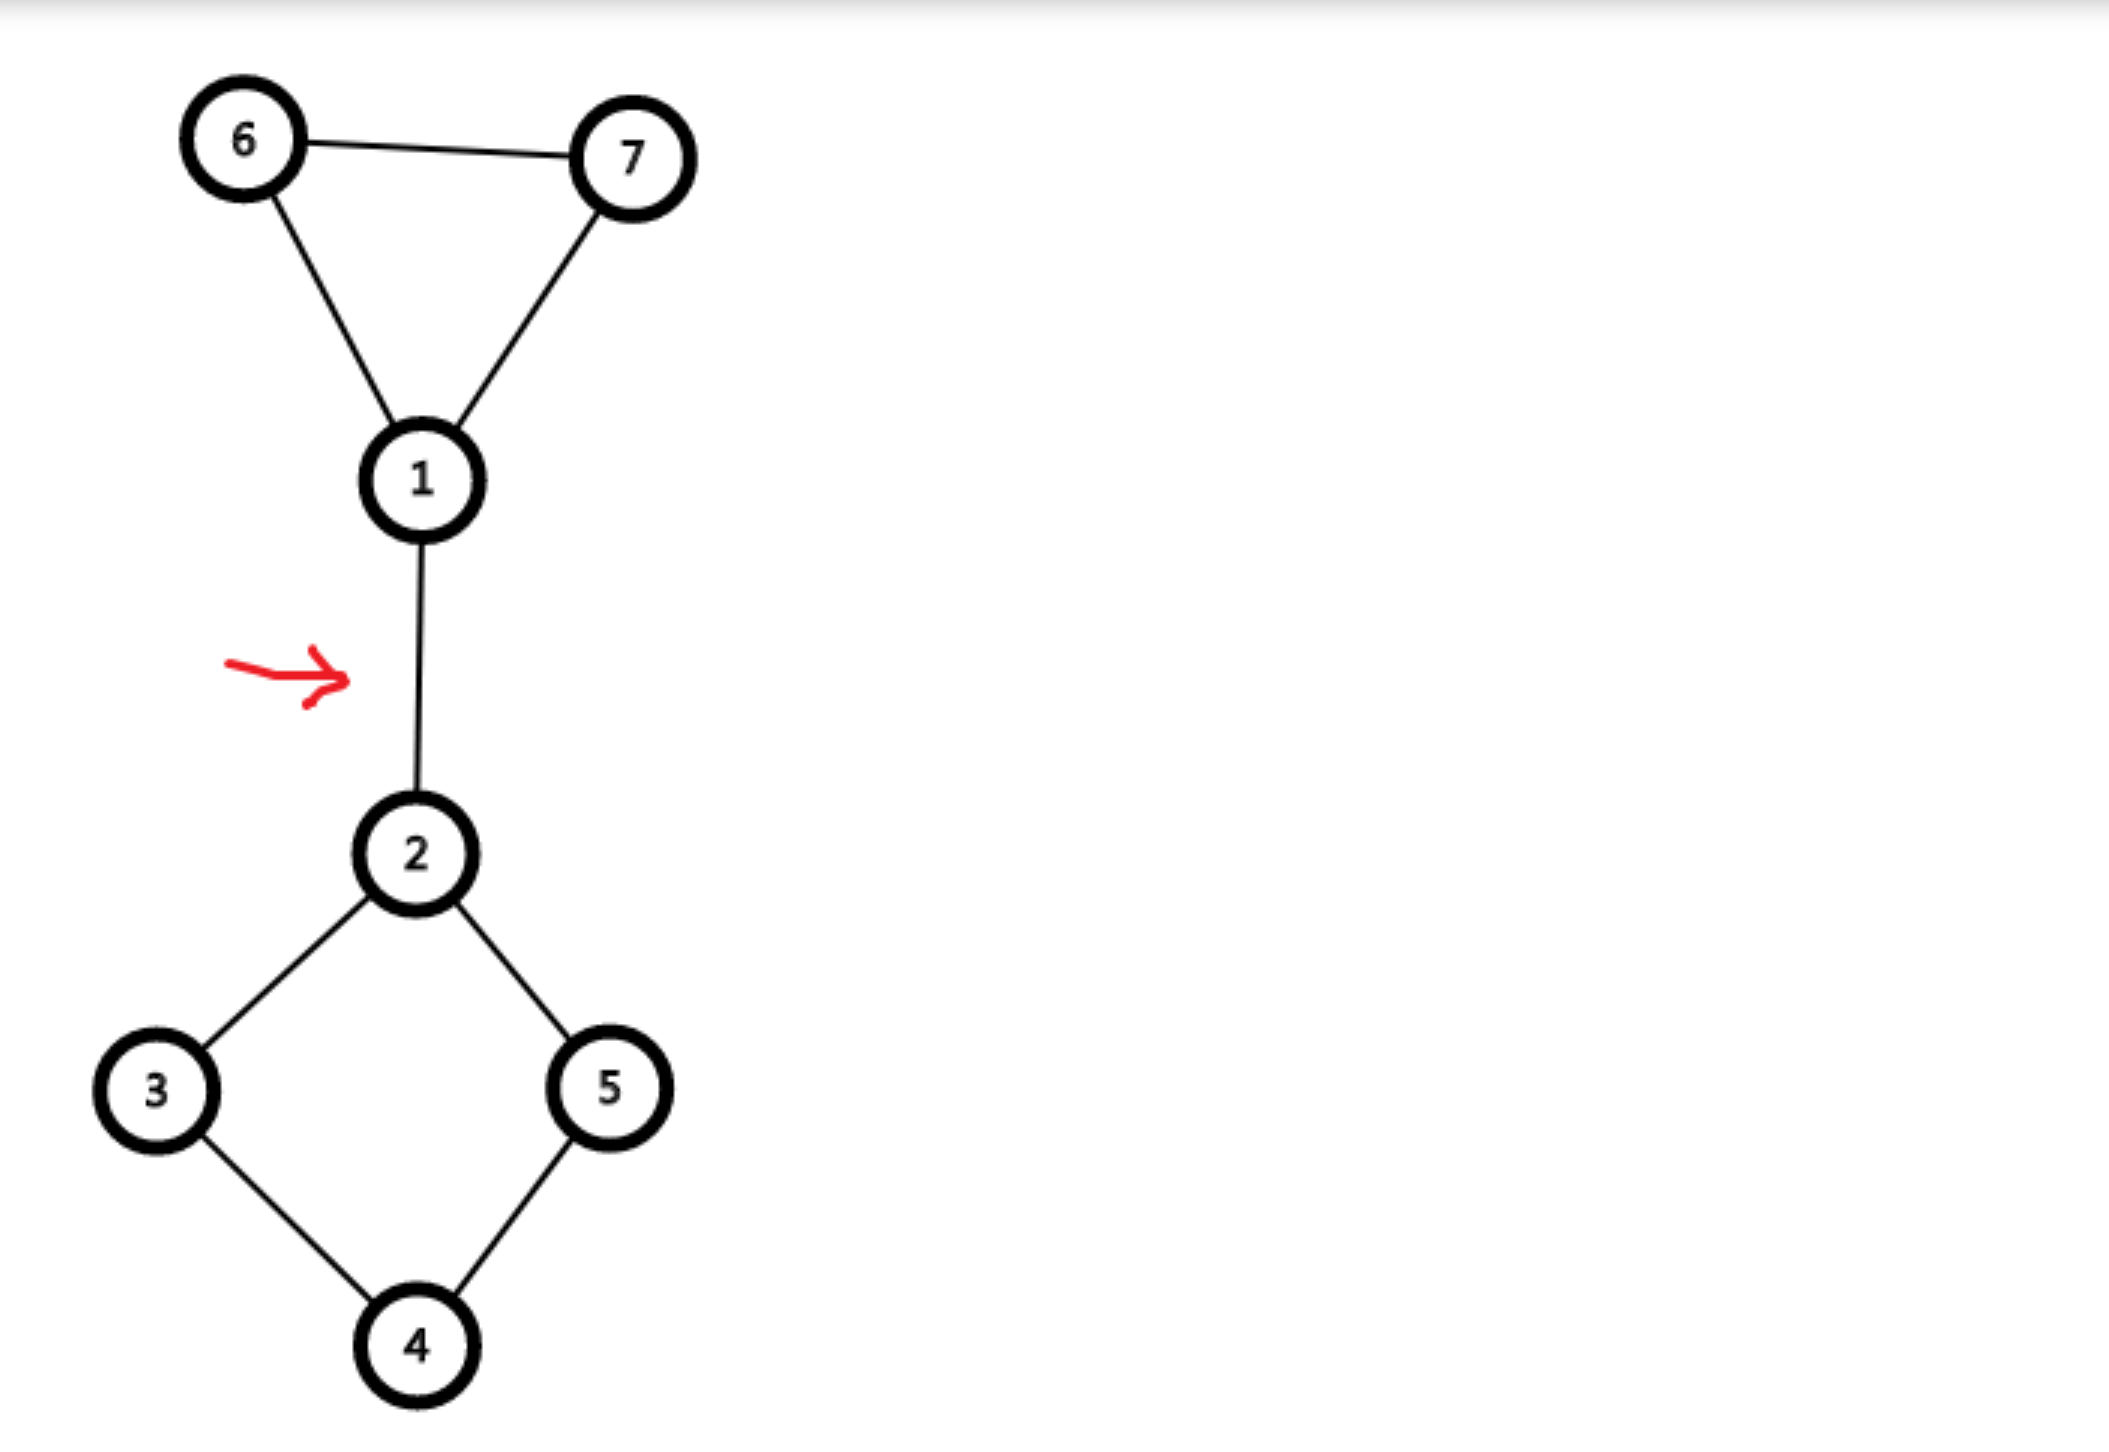
\includegraphics[width=0.95\textwidth]{D:/ACM/代码模板/ver6.0/ICPC-Code-Template-in-Latex/图论/tarjan/bridge4.png}

红色箭头指向的就是割边。

实现

和割点差不多,只要改一处: $low_v>num_u$ 就可以了,而且不需要考虑根节点的问题。

割边是和是不是根节点没关系的,原来我们求割点的时候是指点 $v$ 是不可能不经过父节点 $u$ 为回到祖先节点(包括父节点),所以顶点 $u$ 是割点。如果 $low_v=num_u$ 表示还可以回到父节点,如果顶点 $v$ 不能回到祖先也没有另外一条回到父亲的路,那么 $u-v$ 这条边就是割边。

代码实现

下面代码实现了求割边,其中,当 isbridge[x] 为真时, (father[x],x) 为一条割边。
